% !TEX TS-program = xelatex
% !TEX encoding = UTF-8 Unicode

% -----------------
% START OF PREAMBLE
% -----------------
\documentclass[11pt,a4paper,headinclude=false,footinclude=false]{scrreprt}
\usepackage[a4paper,top=2cm,bottom=2cm,left=3cm,right=3cm]{geometry}

% Commands
\newcommand{\HRule}{\rule{\linewidth}{0.5mm}}


% Packages
\usepackage{fontspec}
\usepackage{eurosym}
\usepackage{amssymb}
\usepackage{mathtools}
\usepackage{upquote}
\usepackage{microtype}
%\usepackage{polyglossia}
\usepackage{longtable,booktabs}
\usepackage{graphicx}
\usepackage{grffile}
\usepackage{ulem}[normalem]
\usepackage{cite}
\usepackage{hyperref}[setpagesize=false,
            unicode=false,
            colorlinks=true,
            urlcolor=blue,
	    linkcolor=black]
\usepackage{float}
\usepackage{tabu}
\usepackage{gensymb}
\usepackage{listings}


% Polyglossia settings
%\setmainlanguage{english} % or danish
%\addto\captionsenglish{%
%  \renewcommand{\contentsname}{Table of Contents}
%}


% Required for syntax highlighting



% Don't let images overflow the page
% Can still explicit set width/height/options for an image
\makeatletter
\def\maxwidth{\ifdim\Gin@nat@width>\linewidth\linewidth\else\Gin@nat@width\fi}
\def\maxheight{\ifdim\Gin@nat@height>\textheight\textheight\else\Gin@nat@height\fi}
\makeatother
\setkeys{Gin}{width=\maxwidth,height=\maxheight,keepaspectratio}


% Make links footnotes instead of hotlinks
\renewcommand{\href}[2]{#2\footnote{\url{#1}}}


% Avoid problems with \sout in headers with hyperref:
\pdfstringdefDisableCommands{\renewcommand{\sout}{}}


% No paragraph indentation
% and set space between paragraphs
\setlength{\parindent}{0pt}
\setlength{\parskip}{1em}
\setlength{\emergencystretch}{3em} % Prevent overfull lines
\renewcommand{\baselinestretch}{1.0}
\pagestyle{plain}
\pagenumbering{arabic}

% -----------------
%  END OF PREAMBLE
% -----------------
\begin{document}


\begin{titlepage}
  \begin{center}

    \textsc{\LARGE Dublin City University}\\[1.5cm]
    \textsc{\Large Electronic and Computer Engineering}\\[0.5cm]

    \HRule\\[0.4cm]
    {\huge \bfseries EE445 Bioelectronics IoT Group Project\\[0.4cm]}
    \HRule\\[1.5cm]

    \begin{figure}[H]
	
\includegraphics{CoverSheet/Dcu-logo.png}
	\centering
    \end{figure}

    \vskip 3cm
    \emph{Authors}\\[0.1cm]
    \noindent\makebox[\textwidth]{%
      \begin{tabular}{ll}%
        Michael Lenehan & michael.lenehan4@mail.dcu.ie \\
	Student Number: & 15410402 \\
	Kiran Chandrath Ravi & kiran.chandrathravi2@mail.dcu.ie\\
	Student Number: & 18212432 \\
	Hanzhu Zhang & hanzhu.zhang@mail.dcu.ie\\
	Student Number: & \\
    \end{tabular}}\\[0.1cm]

    \vfill

    % Bottom of the page
    % Probably replaced with date of deadline
      {\large{08/04/2019}}

  \end{center}
\end{titlepage}


% Chapter: 0, section: 1, subsection: 2 etc
\setcounter{secnumdepth}{1}
\setcounter{tocdepth}{1}
\tableofcontents
\listoffigures
%\end{document}
\hypertarget{introduction}{%
\chapter{Introduction}\label{introduction}}

\hypertarget{aims}{%
\section{Aims}\label{aims}}

The aim of this project is to implement a connected ECG sensing system,
utilising the Texas Instruments MSP432 Microcontroller, and IoT
analytics platform ThingSpeak. The system must take heart rate
measurements, via a designed bioamplifier circuit using the standard
lead configurations, using the MSP432 Microcontroller. These
measurements must then be transmit to ThingSpeak via a HTTP POST
command, at which point they can be analysed using MATLAB scripts on
ThingSpeak. Finally, results must be compared to that of another group.

This project aims to improve the students familiarity with bioamplifier
circuits, measurements of biopotential values, and with connected
services, in the ThingSpeak implementation. The ethical issues
associated with the measurement and storage of biopotential
measurements, and user data in general, must also be considered.

\hypertarget{hardware}{%
\chapter{Hardware}\label{hardware}}

\hypertarget{components}{%
\section{Components}\label{components}}

The three op-amp connection circuit is known as the instrumentation
amplifier. It is one of the key parts of the bio-amplifier where the
major signal amplification and cancelling out of noise takes place. The
input stage of the instrumentation amplifier has a very high input
impedance and low common mode gain and hence it can reject all the
common mode voltages or noises\cite{BioAmp}. The gain stage of the
amplifier produces the differential gain to the signal and also has a
low input impedance and hence for the overall amplifier system it
amplifies only the differential component and has a very high common
mode rejection ration and for rejection of the common mode voltages we
use the driven right leg circuit as illustrated below. The common mode
signal is given as a reference.

\begin{figure}[H]
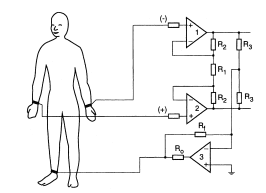
\includegraphics{Images/Hardware/DrivenRightLeg.png}
\centering
\caption{Driven Right Leg Circuit for Common Mode Rejection \cite{tweed}}
\label{drivenright}
\end{figure}

As the instrumentation amplifier we use the IC AD620, which is a low
cost, highly accurate instrumentation amplifier that can set a gain of 1
to 10,000. It has 8 lead SOIC and DIP packing. The diagram and pinout of
AD620 is given below.

\begin{figure}[H]
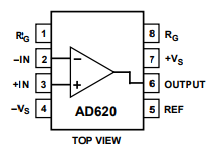
\includegraphics{Images/Hardware/InstrumentationAmplifier.png}
\centering
\caption{AD620 Instrumentation Amplifier Pinout\cite{analog}}
\label{ad620}
\end{figure}

\hypertarget{operationalisolation-amplifier}{%
\subsection{Operational/Isolation
Amplifier}\label{operationalisolation-amplifier}}

These are also known as the pre-amplification circuits. The main purpose
of the isolation amplifier is to provide electrical insulation to the
patient and also prevents internal cardiac shock, and it increases the
input impedance of the patient monitoring system.

\hypertarget{band-pass-filter}{%
\subsection{Band Pass Filter}\label{band-pass-filter}}

As for designing the high pass filter a resistance of \(22k\Omega\) and
a capacitor of \(1\mu F\)is used. The high pass filter is used to
attenuate a signal below a certain frequency range.

\begin{figure}[H]
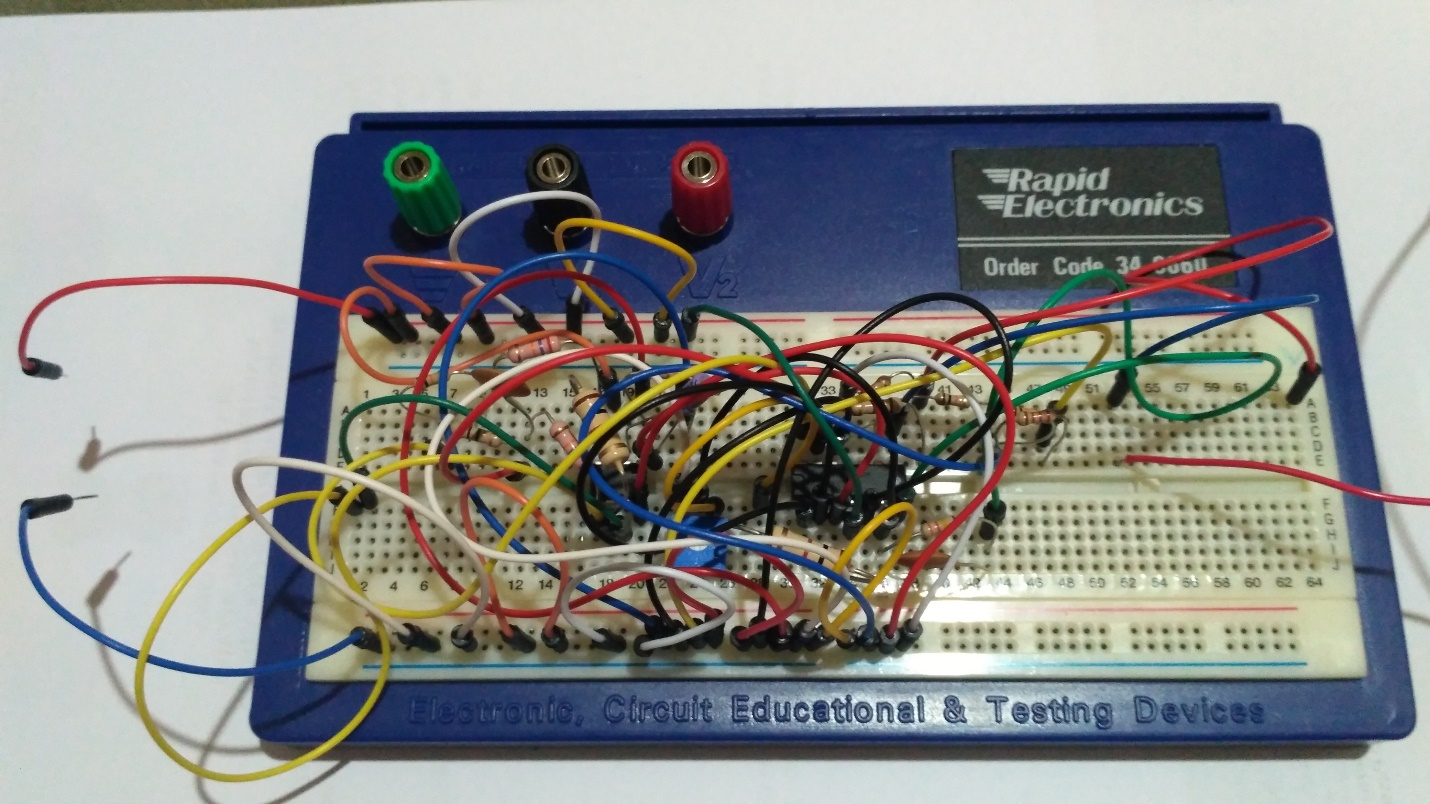
\includegraphics{Images/Hardware/CircuitPhoto.jpg}
\centering
\caption{An Image of the Completed Circuit}
\label{circuitphoto}
\end{figure}

\hypertarget{amplifier-design}{%
\section{Amplifier Design}\label{amplifier-design}}

The key function of a biopotential amplifier is the amplify the weak
electrical signals that has biological origin. Biological signals are
received as potentials, or voltage changes and also as the electrical
field strengths produced by the muscles or nerves. The output signals
from these amplifiers will be of the range \(1\) to \(100mV\)
accompanied with extremely high-level interference signals and noise and
large source impedance. The signal received from the biological origin
is to be amplified and then converted to digital signal for performing
computer manipulations. This amplifier has to provide selective
amplification to the biological signal while detecting and cancelling
all other interference noises and signals and on the other hand should
provide electrical insulation to the subject as well\cite{BioAmp}.
Figure \ref{bioBlock} represents basic model of a bio potential
amplifier. It consists of the following parts:

\begin{enumerate}
\item Preamplifier or the instrumentation amplifier.
\item High pass filters
\item Isolation Amplifier
\item Low-pass filters
\end{enumerate}

\begin{figure}[H]
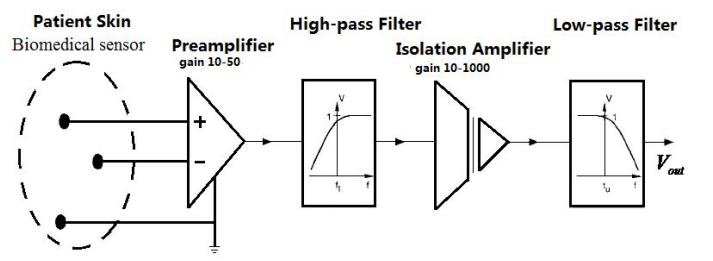
\includegraphics{Images/Hardware/BioamplifierBlockDiagram.png}
\centering
\caption{Bioamplifier Block Diagram}
\label{bioBlock}
\end{figure}

There are some basic requirements that is to be fulfilled while
modelling and using a biopotential amplifier.

\begin{itemize}
\item The signal received should not have any distortion in it.
\item The signal should achieve best separation between the signal, noise and
interference.
\item The amplifier should provide electrical insulation to the patient
\item The amplifier should also protect itself from the high input voltages from
the defibrillators or electrosurgical instrumentation.
\end{itemize}

\begin{figure}[H]
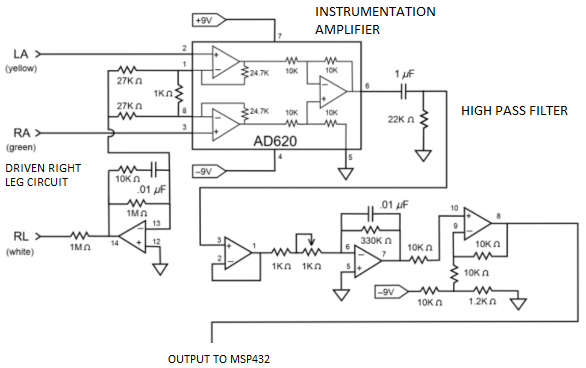
\includegraphics{Images/Hardware/CircuitDiagram.png}
\centering
\caption{Complete Circuit Diagram}
\label{circuitdiagram}
\end{figure}

\hypertarget{software}{%
\chapter{Software}\label{software}}

There are three main aspects to the software portion of this project.
These are the ECG Sampling, the transfer of sampled data to ThingSpeak,
and the MATLAB analysis of the data available on ThingSpeak. Due to
limitations with ThingSpeaks update frequency, proper sampling results
were required to be uploaded in bulk to the site.

\hypertarget{ecg-sampling}{%
\section{ECG Sampling}\label{ecg-sampling}}

The ECG sampling code implementation, as used within this project, was
performed at a frequency of 50Hz (one sample every 20ms). This frequency
was chosen as it allows for the detection of all ECG
components\cite{biopacl5}. However, due to limitations imposed by
ThingSpeak, which could not allow for a frequency greater than one
sample every 15 seconds to be chosen for single data entries. As such
multiple data points must be transmit at once.

In order to take measurements from the bioamplifier circuit, an input
pin must first be defined. An String variable must be defined in order
to store the measured value, along with String to store the reading
times. The sampling frequency time is stored as a constant integer
value.

\lstset{
    caption=Analog Input Pin Definition,
    basicstyle=\footnotesize, frame=tb,
    xleftmargin=.2\textwidth, xrightmargin=.2\textwidth
}
\begin{lstlisting}[language=C]
int AnalogPin = A6; //P4.7
String reading;
String readtime;
int index = 0;
const int updateReading = 20;
\end{lstlisting}

In order to take the reading, the analogRead() method must be called.
This method allows the MSP to read in analog values from 0 to 5V,
assigning them a value between 0 and 1023. An if statement is used to
ensure that the readings are taken at the appropriate timing. The time
of each reading is stored, along with the time the reading is taken. The
index is incremented on each reading. As 750 readings may be taken at
20ms intervals over a period of 15 seconds, the index will be reset
after the 749th reading.

\lstset{
    caption=Analog Read,
    basicstyle=\footnotesize, frame=tb,
    xleftmargin=.1\textwidth, xrightmargin=.1\textwidth
}
\begin{lstlisting}[language=C]
if(millis() - lastReadingTime > updateReading){
    reading = reading+String(analogRead(AnalogPin))+" ";
    readtime = readtime+String(millis())+" ";
    ...
    lastReadingTime = millis();
    if(index<749){index = index+1;}
    else {
    index=0;
    reading="";
    readtime="";
    }
}
\end{lstlisting}

\hypertarget{thingspeak-integration}{%
\section{ThingSpeak Integration}\label{thingspeak-integration}}

ThingSpeak integration is performed using the ThingSpeakClient.ino code
example found in the Energia git repository\cite{thingino}. This example
works much in the same way as the Energia WifiWebClient example code,
however, it has code included to update ThingSpeak input fields, in the
required format.

In order to correctly utilize this code, the ThingSpeak write API key
must be included in the code, as a String value. An update interval
value is used in order to set how often data is sent to ThingSpeak from
the client. For this implementation, this has been set to 15 seconds, as
this was the lowest accepted value.

\lstset{
    caption=ThingSpeakClient.ino write API key and update interval,
    basicstyle=\footnotesize, frame=tb,
    xleftmargin=.1\textwidth, xrightmargin=.1\textwidth
}
\begin{lstlisting}[language=C]
String writeAPIkey = ""; //Enter channel's write API key
                        //between the ""
const int updateThingSpeakInterval = 15*1000; //20ms time interval
\end{lstlisting}

The startWiFi() method is called from within the codes setup, and
connects to the network of the input ssid and password, printing a
success message to the serial monitor once connected.

\lstset{
    caption=ThingSpeakClient.ino startWifi(),
    basicstyle=\footnotesize, frame=tb,
    xleftmargin=.1\textwidth, xrightmargin=.1\textwidth
}
\begin{lstlisting}[language=C]
char ssid[] = ""; // your network SSID (name)
char pass[] = ""; // your network password
WiFiClient client;
void startWiFi(){
    WiFi.disconnect();
    client.stop();
    ...
    if(WiFi.begin(ssid, pass) == 0){
    ...
    } else {
    Serial.println("LaunchPad connected to network using DHCP");
    ...
    }
}
\end{lstlisting}

Within the loop function, an if statement checks for connection to the
client, and reads any incoming response. If no client is connected, a
disconnection notification is printed to the serial monitor.

Another if statement checks if the update interval has been exceeded,
and, if so, writes data via HTTP POST message to ThingSpeak, using the
updateThingSpeak() method.

\lstset{
    caption=ThingSpeakClient.ino Loop Function,
    basicstyle=\footnotesize, frame=tb,
    xleftmargin=.1\textwidth, xrightmargin=.1\textwidth
}
\begin{lstlisting}[language=C]
long lastConnectionTime = 0;
boolean lastConnected = false;
void loopThingSpeakClient(){
    if(client.available()){
    char c = client.read();
    Serial.println(c);
    }
    if(!client.connected() && lastConnected){
    Serial.println("...disconnected");
    ...
    client.stop();
    }
    if(!client.connected() && (millis() - lastConnectionTime >
    updateThingSpeakInterval)) {
    String updateVal = "field1="+reading+",field2="+readtime;
    updateThingSpeak(updateVal);
    }
    ...
    lastConnected = client.connected();
}
\end{lstlisting}

The updateThingSpeak() method ensures that the device is correctly
connected to the website, and transmits the ECG readings via HTTP POST
message. If the transfer fails, the client disconnects.

\lstset{
    caption=ThingSpeakClient.ino updateThingSpeak Function,
    basicstyle=\footnotesize, frame=tb,
    xleftmargin=.1\textwidth, xrightmargin=.1\textwidth
}
\begin{lstlisting}[language=C]
void updateThingSpeak(String tsData){
    if(clinet.connect(thingSpeakAddress, 80)){
    ...
    client.print("POST /update HTTP/1.1\n");
    client.print("Host: api.thingspeak.com\n");
    client.print("Connection: close\n");
    client.print("X-THINGSPEAKAPIKEY: " + writeAPIkey + "\n");
    client.print("Content-Type: application/x-www-form-urlencoded\n");
    client.print("Content-Length: ");
    client.print(tsData.length());
    client.print("\n\n");
    client.print(tsData);
    ...
    failedCounter = 0;
    } else {
    failedCounter++;
    client.stop();
    ...
    }
    lastConnectionTime = millis();
}
\end{lstlisting}

\hypertarget{matlab-script}{%
\section{MATLAB Script}\label{matlab-script}}

The MATLAB script used for data visualisation within ThingSpeak is
required to read in data from two strings, convert them from the
``table'' format in which they are sent from the client device, and
split the string by whitespace, and plot the data from the time string
against the ECG data string.

\lstset{
    caption=ThingSpeak MATLAB Code,
    basicstyle=\footnotesize, frame=tb,
    xleftmargin=.1\textwidth, xrightmargin=.1\textwidth
}
\begin{lstlisting}[language=C]
readChannelID = 767748;
fieldID1 = 1;
fieldID2 = 2;
readAPIKey = ''; %Enter Read API Key between ''

[data, dataTime time] = thingSpeakRead(readChannelID, 'Field', fieldID1,
'Field', fieldID2, 'NumPoints', 1, 'ReadKey', readAPIKey, 'OutputFormat',
'table')

%% Data must be modified to a matrix of integer values.
%% This requires the data to be made into a table using:

dataTable = table(data.ECGData);
dataTimeTable = table(data.ECGTimes);

%% Table must be converted to array

dataArray = table2array(dataTable);
dataTimeArray = table2array(dataTimeTable);

%% Cell Array must be converted to matrix

dataMat = cell2mat(dataArray);
dataTimeMat = cell2mat(dataTimeArray);

%% Each Value of the String must be split by a whitespace delimiter

dataSplit = strsplit(dataMat(1,1:end));
dataTimeSplit = strsplit(dataTimeMat(1,1:end));

%% Split Cells must be converted to matrix

dataSplitMat = [dataSplit(:)];
dataTimeSplitMat = [dataTimeSplit(:)];

%% Convert String values to Double

dataFinalMat = cellfun(@str2double, dataSplitMat);
dataTimeFinalMat = cellfun(@str2double, dataTimeSplitMat);

%% Plot Time values versus Data values

plot(dataTimeFinalMat, dataFinalMat);
\end{lstlisting}

In order to acquire data from another groups channel, for comparison,
the channel ID and read API key would be required. The comparison could
be made by taking the difference of both ``dataFinalMat'' variables,
assuming each group has uploaded their value in the same manner.
Unfortunately, this implementation was not completed.

\hypertarget{possible-improvements}{%
\section{Possible Improvements}\label{possible-improvements}}

Due to the limitations imposed by ThingSpeak, the maximum available
sampling rate, when uploading one data sample at a time is 1 sample
every 15 seconds. However, the implementation used, uploading bulk data
via a single string causes a number of functions to be performed on the
data structure, in order for it to be in a usable format for plotting
and comparison. An alternative approach would involve using the JSON
message format to send bulk data, along with the timestamp of each data
point\cite{matlabbulk}. Using this, a more simple plot function could be
performed from within the MATLAB code, as only one field within the
channel would be used, with the appropriate data points and timestamps
contained within it.

\hypertarget{ethics}{%
\chapter{Ethics}\label{ethics}}

There are a number of ethical issues associated with the capture and
storage of personal data. Uploading data using the implementation in
this project, data could be intercepted, allowing the person
intercepting it access to all of the data. Data should be uploaded by
more secure means, and stored in an encrypted format. This would prevent
any data which may be intercepted from being used. The data being stored
is also not being stored with personal data protection regulations, such
as GDPR, in mind. A more complete solution would allow for encrypted
data to be uploaded, and would store this data in a secure way, not
easily accessible.
\bibliography{References/biblio}{}
\bibliographystyle{IEEEtran}
\end{document}
